% Fig. 2: AQPS closed-loop architecture. Compile: pdflatex fig2_architecture.tex (standalone)
\documentclass[tikz,border=2pt]{standalone}
\usepackage{mathptmx}
\usetikzlibrary{arrows.meta,positioning,calc}
\definecolor{ink}{HTML}{1F1F1F}
\definecolor{ink2}{HTML}{555555}
\definecolor{blu}{HTML}{2A78D6}
\definecolor{red}{HTML}{E34948}
\definecolor{yel}{HTML}{EDA100}
\begin{document}
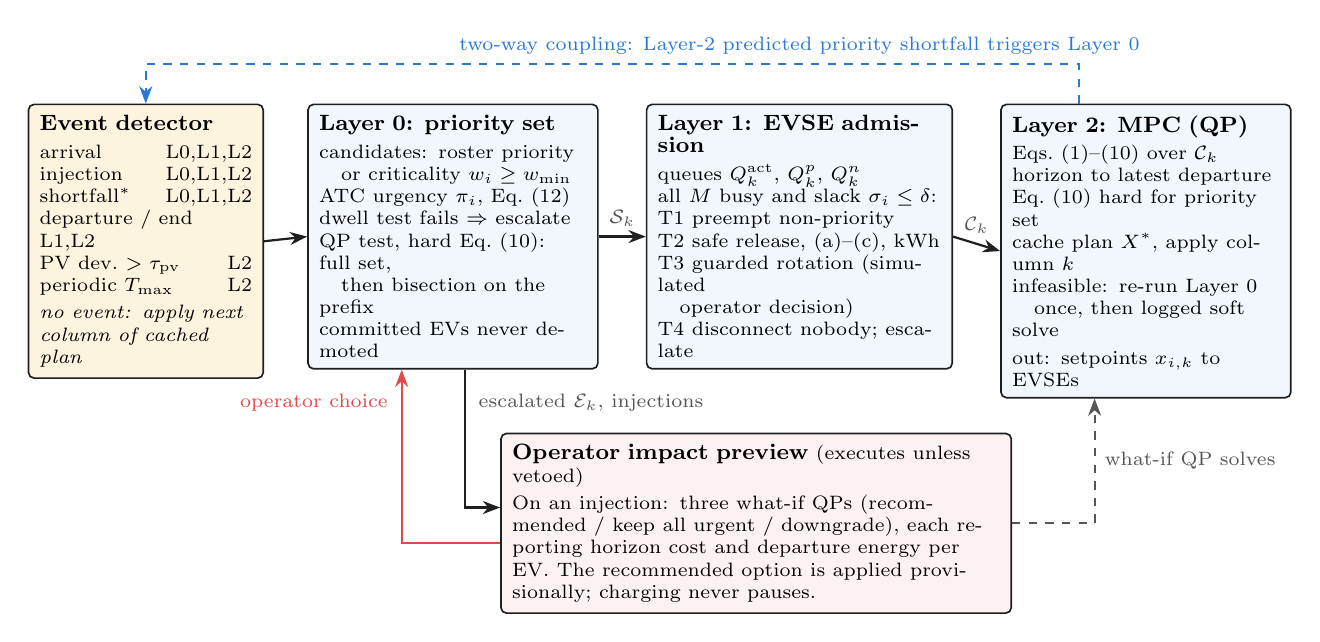
\begin{tikzpicture}[
  >={Stealth[length=2.2mm]}, line width=0.6pt,
  box/.style={draw=ink, rounded corners=2pt, align=left, inner sep=4pt, font=\scriptsize,
              text width=#1, minimum height=33mm, anchor=north west},
  flow/.style={->, draw=ink, line width=0.8pt},
  lab/.style={font=\scriptsize, ink2},
]
\def\top{0}
\node[box=27mm, fill=yel!12] (evt) at (0,\top) {%
  {\footnotesize\bfseries Event detector}\\[2pt]
  arrival \hfill L0,L1,L2\\
  injection \hfill L0,L1,L2\\
  shortfall$^{\ast}$ \hfill L0,L1,L2\\
  departure / end \hfill L1,L2\\
  PV dev.\ $>\tau_\mathrm{pv}$ \hfill L2\\
  periodic $T_\mathrm{max}$ \hfill L2\\[2pt]
  \textit{no event: apply next}\\
  \textit{column of cached plan}};
\node[box=34mm, fill=blu!6] (l0) at (3.55,\top) {%
  {\footnotesize\bfseries Layer 0: priority set}\\[2pt]
  candidates: roster priority\\ \quad or criticality $w_i\ge w_\mathrm{min}$\\
  ATC urgency $\pi_i$, Eq.~(12)\\
  dwell test fails $\Rightarrow$ escalate\\
  QP test, hard Eq.~(10): full set,\\ \quad then bisection on the prefix\\
  committed EVs never demoted};
\node[box=36mm, fill=blu!6] (l1) at (7.85,\top) {%
  {\footnotesize\bfseries Layer 1: EVSE admission}\\[2pt]
  queues $Q^{\mathrm{act}}_k$, $Q^{p}_k$, $Q^{n}_k$\\
  all $M$ busy and slack $\sigma_i\le\delta$:\\
  T1 preempt non-priority\\
  T2 safe release, (a)--(c), kWh\\
  T3 guarded rotation (simulated\\ \quad operator decision)\\
  T4 disconnect nobody; escalate};
\node[box=34mm, fill=blu!6] (l2) at (12.35,\top) {%
  {\footnotesize\bfseries Layer 2: MPC (QP)}\\[2pt]
  Eqs.~(1)--(10) over $\mathcal{C}_k$\\
  horizon to latest departure\\
  Eq.~(10) hard for priority set\\
  cache plan $X^\ast$, apply column $k$\\
  infeasible: re-run Layer 0\\ \quad once, then logged soft solve\\[2pt]
  out: setpoints $x_{i,k}$ to EVSEs};
\node[draw=ink, rounded corners=2pt, fill=red!7, align=left, font=\scriptsize, text width=62mm, inner sep=4pt,
  anchor=north west] (op) at ($(l0.south west)+(2.45,-0.8)$) {%
  {\footnotesize\bfseries Operator impact preview} (executes unless vetoed)\\[2pt]
  On an injection: three what-if QPs (recommended / keep all urgent / downgrade), each reporting horizon
  cost and departure energy per EV. The recommended option is applied provisionally; charging never pauses.};
\draw[flow] (evt.east) -- (l0.west);
\draw[flow] (l0.east) -- node[lab, above] {$\mathcal{S}_k$} (l1.west);
\draw[flow] (l1.east) -- node[lab, above] {$\mathcal{C}_k$} (l2.west);
\draw[->, draw=blu, dashed, line width=0.8pt] ([xshift=10mm]l2.north west) -- ++(0,5mm) -| ([xshift=15mm]evt.north west);
\node[font=\scriptsize, blu, anchor=south] at ($(l1.north)+(0,5mm)$) {two-way coupling: Layer-2 predicted priority shortfall triggers Layer 0};
\draw[flow] ([xshift=20mm]l0.south west) |- ([yshift=2mm]op.west);
\node[lab, anchor=west] at ($(l0.south west)+(2.05,-0.42)$) {escalated $\mathcal{E}_k$, injections};
\draw[flow, draw=red] ([yshift=-2.5mm]op.west) -| ([xshift=12mm]l0.south west);
\node[lab, anchor=east, text=red] at ($(l0.south west)+(1.15,-0.42)$) {operator choice};
\draw[->, draw=ink2, dashed, line width=0.7pt] (op.east) -| node[lab, pos=0.75, right] {what-if QP solves} ([xshift=12mm]l2.south west);
\end{tikzpicture}
\end{document}
